\chapter{Tests unitaires}

Suite au choix que nous avons réalisé dans la partie précédente, nous avons commandé notre matériel. Dès la réception de celui-ci nous avons effectué des tests unitaires pour vérifier leur bon fonctionnement. Voici la liste de l'ensemble des tests que nous avons réalisés.



%%%%%%%%%%%%%%%%%%%%%%%%%%%%%%%%%%%%%%%%%%%%%%%%%%%

\section{PIC}
\label{sec:pic}

Dans le schéma du Montréal 3v2 nous avons pu constater qu'il y avait 3 PIC programmés. Nous avons commandé les PIC programmés au près de l'entreprise F1LVT \cite{montreal}.


\begin{figure}[!h]
  \centering
  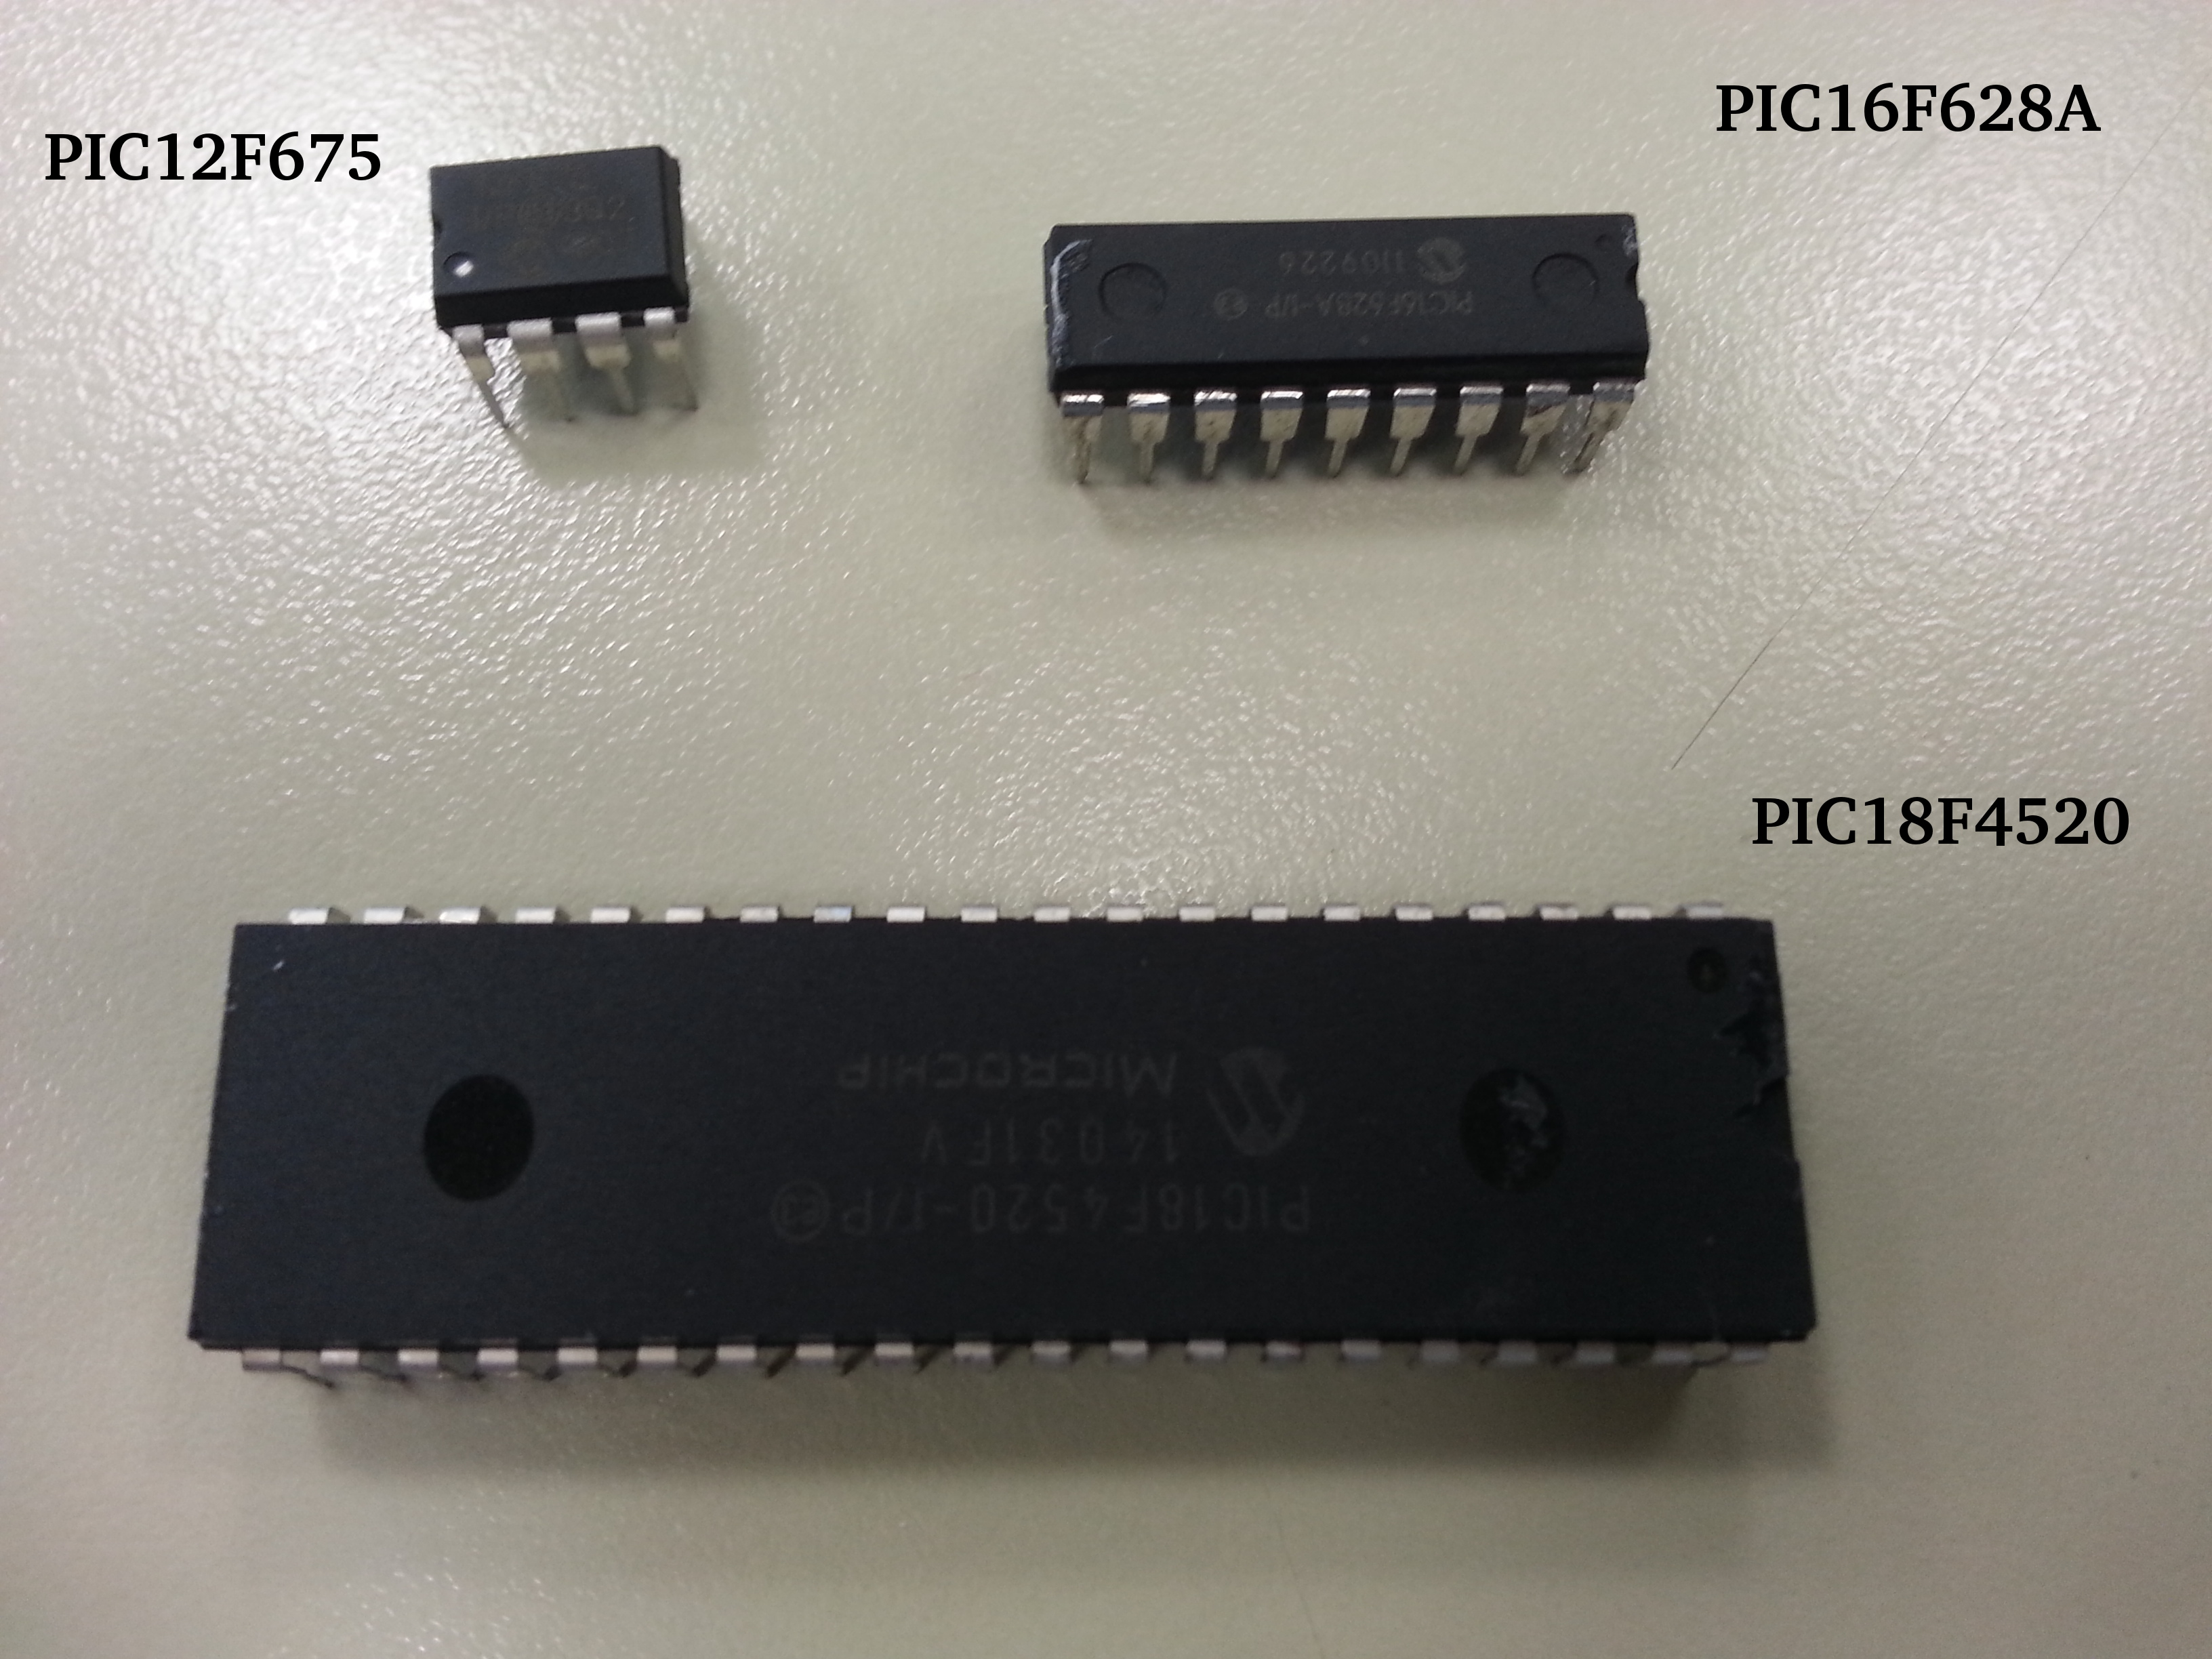
\includegraphics[width=\textwidth]{Test_unitaire/Pic/pic}
  \caption{3 PIC programmés}
  \label{fig:pic}
\end{figure}

Nous avons ensuite imaginé et réalisé des tests unitaires sur chacun des PIC pour vérifier qu'ils ont bien été programmés et qu'aucune erreur n'est apparue sur ce système de décision critique pour le système.

\subsection{PIC16F628A}
\label{sec:picled}

Ce PIC sert à réaliser l'affichage sur les LED. Pour tester ce PIC, nous avons réalisé le montage de la figure \ref{fig:picled}. On peut voir à la figure \ref{fig:schemapic} le schéma de montage du PIC sur le Montréal 3v2.

\begin{figure}[!h]
  \centering
  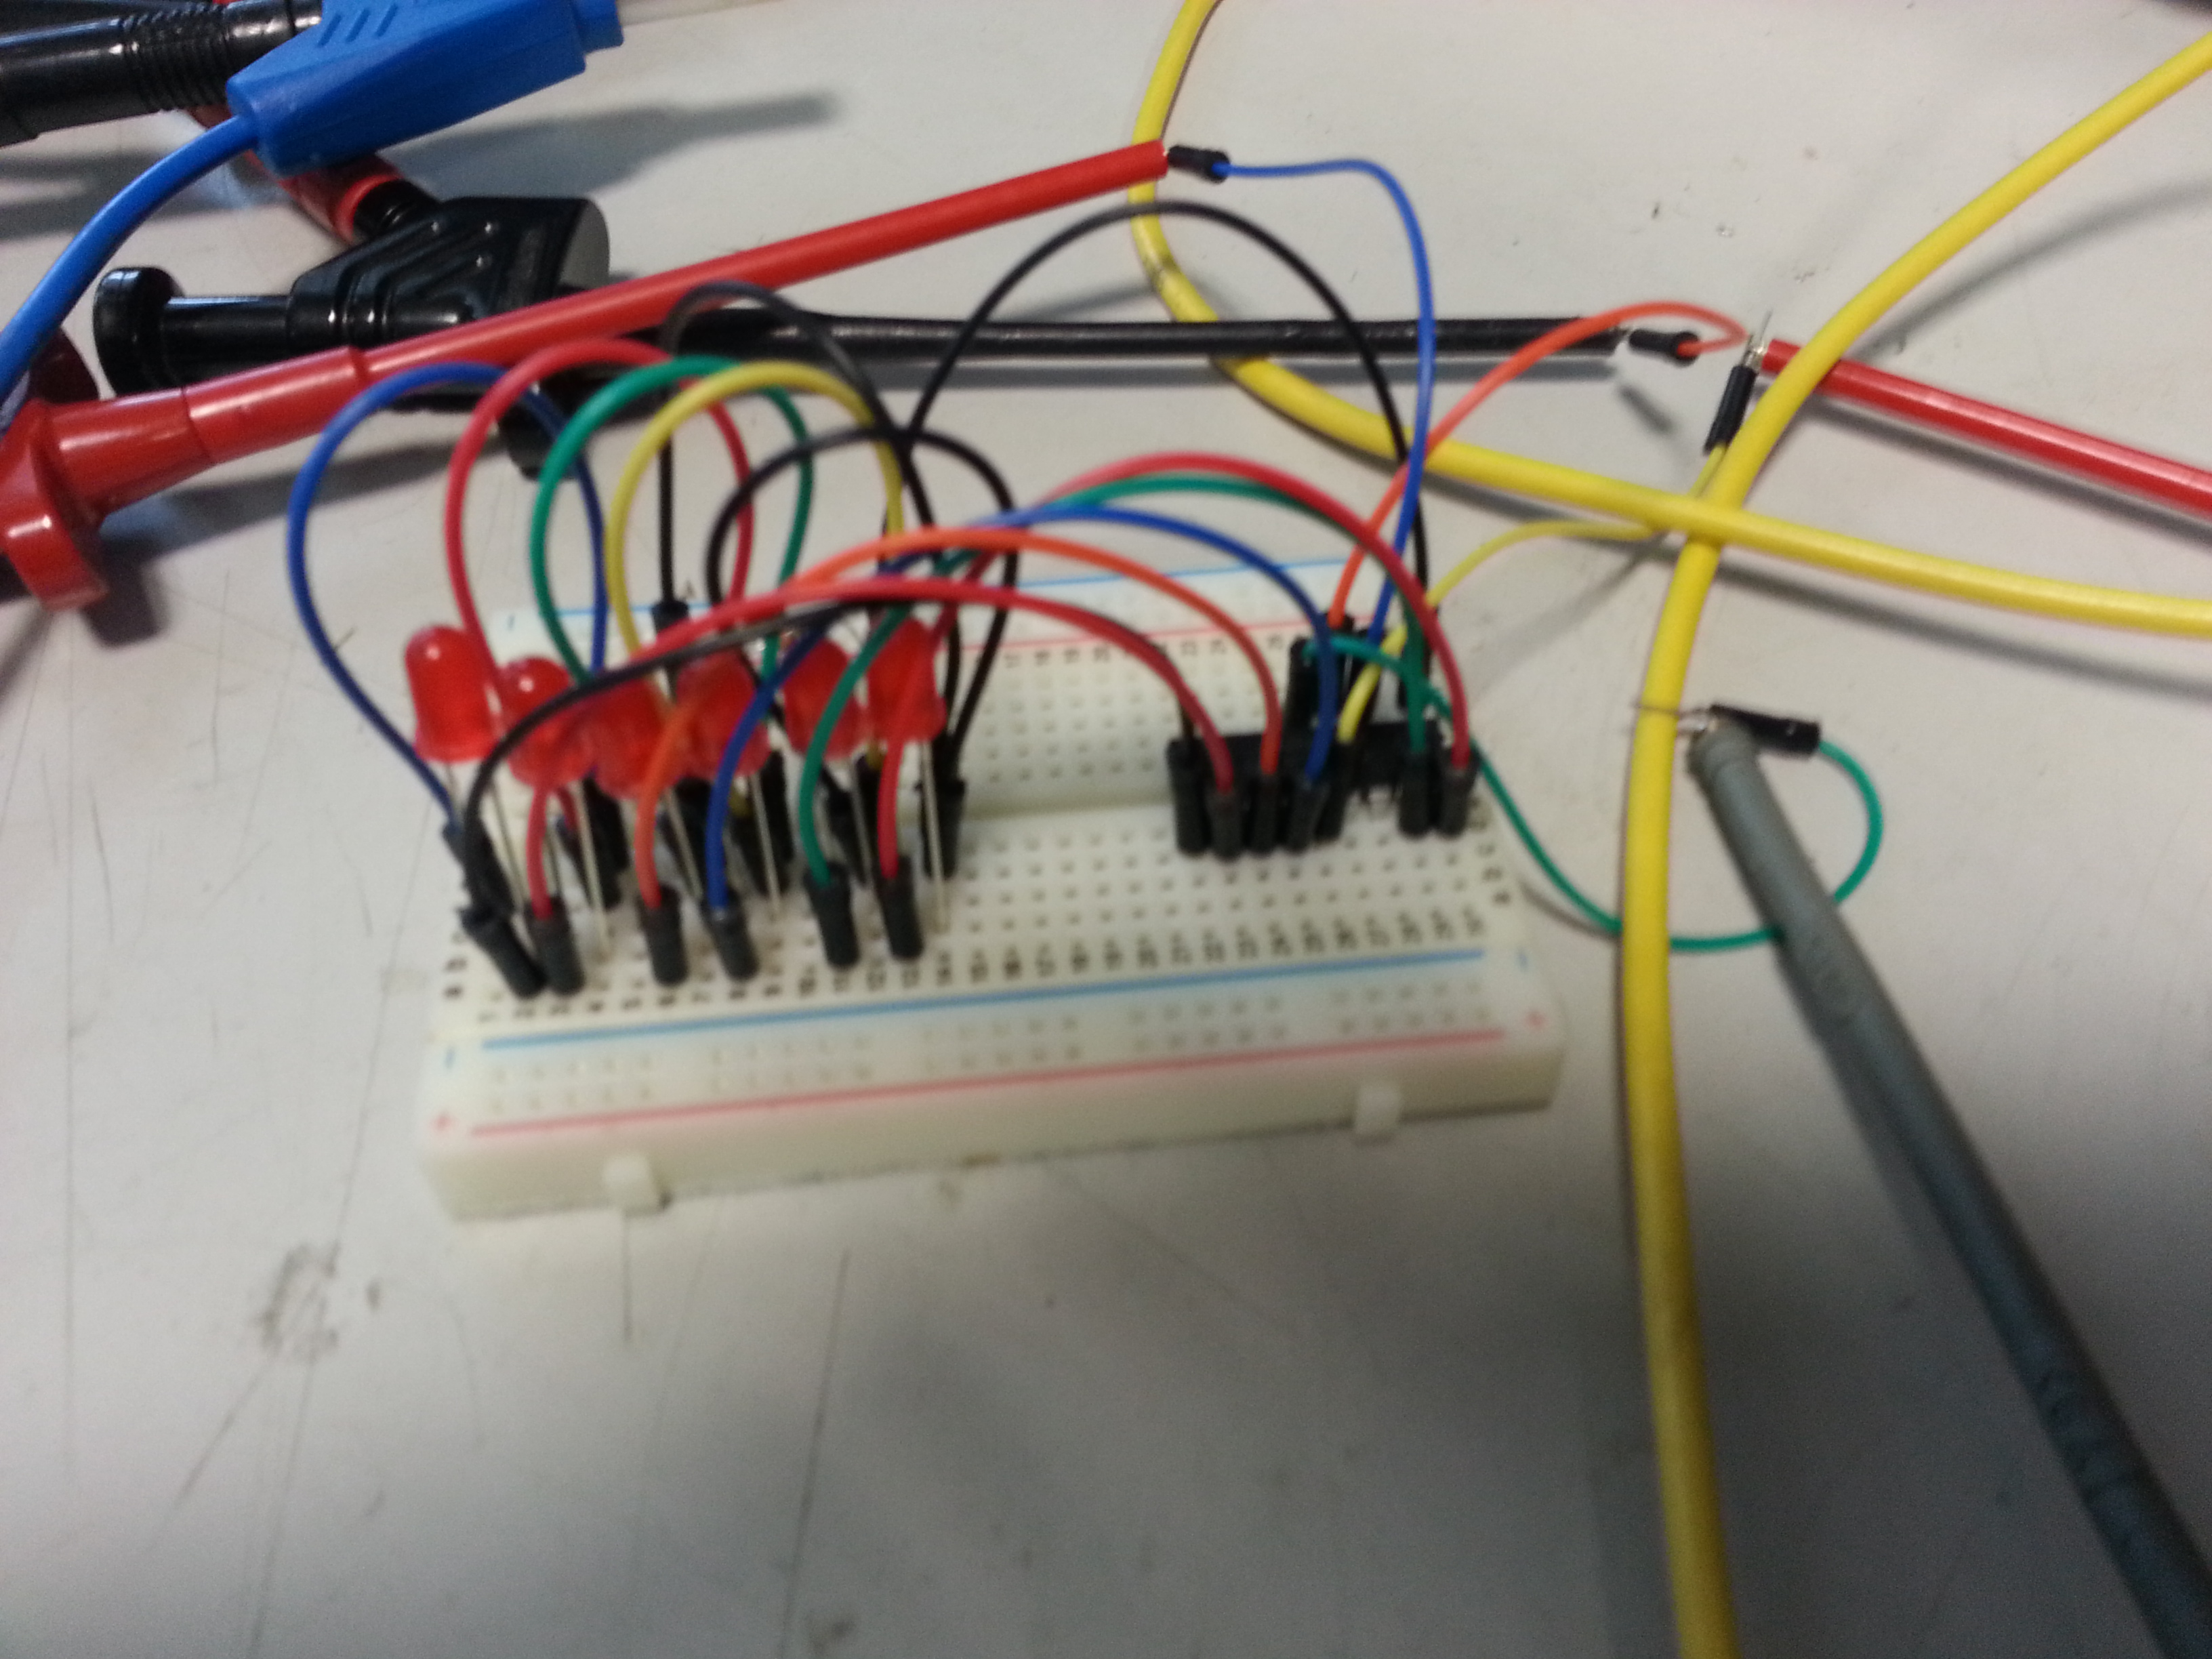
\includegraphics[width=\textwidth]{Test_unitaire/Pic/picled}
  \caption{Schéma electrique du test unitaire}
  \label{fig:picled}
\end{figure}


Pour tester ce composant, nous avons donc choisi de monter une partie des LED situées en sortie, de configurer le \og clock\fg{} sur un signal carré de fréquence 1 MHz, et de faire varier la fréquence de l'entrée \og data\fg{}.

Malheureusement nous n'avons pas pu observer de LED s'allumer pendant notre expérience.

\begin{figure}[!h]
  \centering
  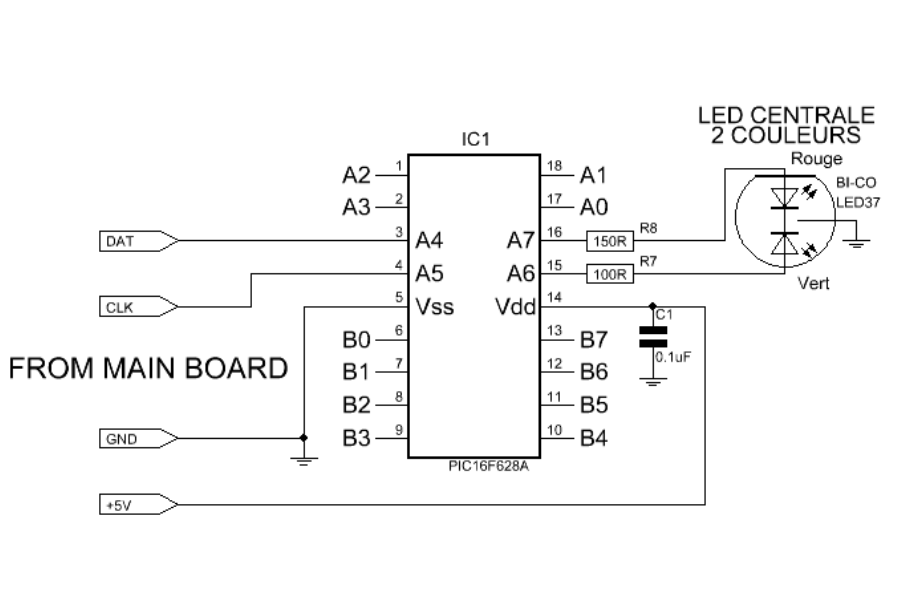
\includegraphics[width=\textwidth]{Test_unitaire/Pic/schemapic}
  \caption{Schéma de montage du pic sur le Montréal 3v2}
  \label{fig:schemapic}
\end{figure}
\newpage
\subsection{PIC12F675 et PIC18F4520}
\label{sec:picclock}


Ces deux PIC ont également été testés avec le même procédé. Nous ne développerons pas plus ces tests car ils nous ont donné les même résultats.

\section{Filtre passe bande}
\label{sec:passe_bande}


Pour le filtre passe bande, nous souhaitions un filtre qui couperait tout ce qui se trouve en dehors de notre bande. Les tests ont montrés que ce filtre réagit plutôt bien quand le montage qui y est lié est adapté, ce qui est le cas, le circuit fonctionne bien avec une impédance de 50 Ohm.

Le test unitaire était simple on a branché le filtre sur un analyseur qui envoyait et recevait un même signal. Il est alors simple d’obtenir le comportement du filtre en observant le signal retour. Nous avons observé que le filtre atténuait très bien ce qui se trouve avant 2.4GHz mais plutôt mal ce qui vient après 2.5GHz. Ceci n’est pas gênant car les bande de fréquences entre 2.5Ghz et 5 GHz sont peu utilisées en France. 

\begin{figure}[h]
  \centering
  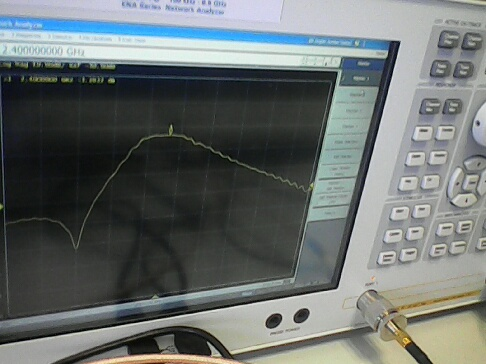
\includegraphics[width=0.8\textwidth]{oscillo1}
  \caption{Comportement du filtre}
  \label{fig:comportement}
\end{figure}

Sur la photo le curseur sur la courbe est à 2.45Ghz et le plat est un peu plus grand que la bande.

Nous avons mesuré deux paramètres supplémentaires, Le S11 et le S21 qui sont des paramètres permettant de mesurer la perte d’amplitude lié au composant. Le S11 est le coefficient de réflexion à l'entrée lorsque la sortie est adaptée. Dans l’idéal il vaut 0, il n’y a alors aucune réflexion et tout l’amplitude du signal sort du filtre, on obtient le S11 de la photo suivante.

On peut voir ici que le log du S11 est très faible entre 2.4 et 2.5 GHz ce qui indique un faible taux de réflexion et donc que le signal en entrée sera peu atténué.

\begin{figure}[h]
  \centering
  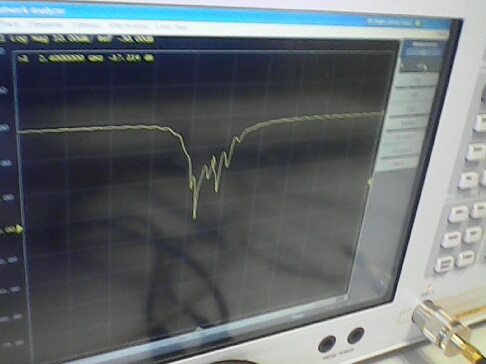
\includegraphics[width=0.8\textwidth]{oscillo2}
  \caption{S11 du filtre passe bande}
  \label{fig:filtre}
\end{figure}


Les deux plus grands pics vers le bas correspondent aux limites de la bande 2.4-2.5GHz.

Le S21 est le coefficient de transmission direct lorsque la sortie est adaptée, pour celui-ci le but est d’avoir ce nombre le plus proche de 1 et donc son logarithme le plus proche de zéro possible.

Lors du test, nous avions une perte d’environ 2dBm dans la bande de fréquence 2.4-2.5GHz, ce qui est relativement faible, le filtre ne risque donc pas d’occulter ce que l’on souhaite voir en atténuant trop fortement le signal utile.
\newpage
\section{VCO}



Le test du VCO est simple mais doit être bien fait car sans lui impossible d’obtenir la bonne fréquence de travail en entrée du radio-goniomètre.

Nous avons commencé par mesurer la fréquence libre, c’est-à-dire la fréquence renvoyée par le VCO lorqu'il est alimenté avec une tension nulle en entrée. La fréquence libre mesurée sur notre matériel était de 1.35 GHz donc plus importante que la fréquence indiqué par le constructeur (1.31Ghz). L'étape suivante consistait à mesurer la tension pour laquelle nous obtenions une fréquence de sortie de 1.9Ghz. Nous avons obtenu environ 8V ce qui nous a permis de choisir le bon régulateur de tension pour la suite.
 Les régulateur sont des composants calibrés, il est donc difficile d’en trouver un qui correspond parfaitement aux besoins du projet. Nous avons heureusement pu obtenir un régulateur à 8.1V qui, après test, permettait d'obtenir en sortie du VCO à une fréquence de 1.91GHz. La bande de fréquence a transférer étant de 100 MHz, donc très large par rapport aux 10MHz de décalage observés initialement, nous avons conservé ce régulateur.


\begin{figure}[h]
  \centering
  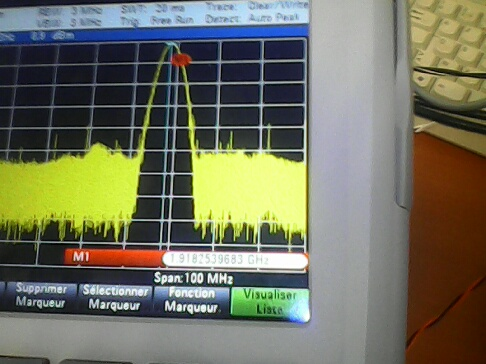
\includegraphics[width=0.8\textwidth]{oscillo3}
  \caption{Fréquences généré par le VCO alimenté à 8.1V centrée autour de 1.9GHz d’une largeur d’environ 10MHz}
  \label{fig:freq}
\end{figure}
\newpage
\section{Down converter}
\label{sec:down_converter}



\begin{figure}[h]
  \centering
  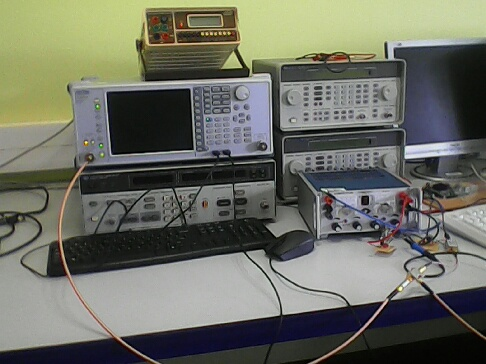
\includegraphics[width=0.8\textwidth]{oscillo4}
  \caption{Montage de test de l’adaptateur}
  \label{fig:mont}
\end{figure}


Le test du down-converter a posé quelques problèmes. Il est nécessaire de l’alimenter comme dans sa configuration opérationnelle et ceci ne peut se faire sans le VCO. De plus le bruit en sortie du VCO risque de gêner l’observation, il est donc obligatoire d'utiliser le filtre.


\begin{figure}[h]
  \centering
  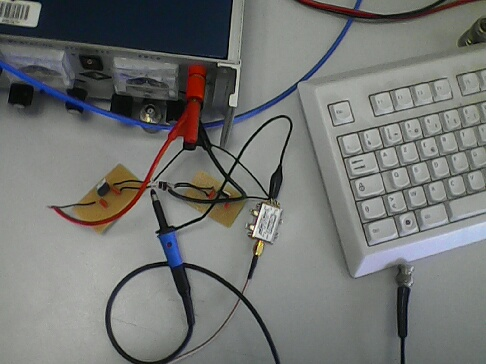
\includegraphics[width=0.8\textwidth]{oscillo5}
  \caption{Photo du VCO et de son alimentation}
  \label{fig:photo}
\end{figure}



Nous avons rencontré différents  problèmes lors du test. Premièrement, des problèmes de communication entre membres de l’équipe ont retardé le test d’une semaine, en effet il a fallu créer un montage avec les deux régulateurs de tension, celui pour l’alimentation et celui pour la tension en entrée. Il manquait cependant une information relative à l'orientation d'un composant sur les schémas fournis au membre de l'équipe chargé de la soudure. Cela a entrainé une erreur de montage avec une augmentation des délais liés à la réalisation de ces filtres.

Deuxièmement, nous n’avions pas prévu des problèmes dus aux câbles. Nous n'étions pas certains que le câblage utilisé n'endommagerait pas le matériel.

Troisièmement, le professeur nous ayant aidé lors de la conception théorique du montage était en déplacement, il n’était donc pas en mesure de nous aider lorsque des hésitations se sont fait sentir. Devant le prix du matériel et la possibilité de l'abimer, nous avons choisi d'attendre.


%%% Local Variables: 
%%% mode: latex
%%% TeX-master: "../rapport"
%%% End: 
